\documentclass{llncs}

\usepackage{graphicx}
\usepackage{url}
\usepackage{courier}
\usepackage{listings}
\usepackage{enumerate}


%!TEX root = ./paper1.tex

\lstset{
  float=tb,
	captionpos=b,
	breaklines=true,
	xleftmargin=20pt,
	basicstyle=\ttfamily\scriptsize,
	numberstyle=\tiny,
	flexiblecolumns=true,
	numbers=left,
	nolol=false,
	tabsize=2
}

\lstdefinelanguage{OCL}{
morekeywords={import,if,then,else,endif,self,and,true,false,def,includes,OclElement,package,let,in},
sensitive=true,
morecomment=[l]{--},
morestring=[b]",
morestring=[b]',
showstringspaces=false
}

\lstdefinelanguage{QVTo}{
morekeywords={import,modeltype,uses,transformation,inout,in,out,configuration,property,main,var,if,then,else,endif,map,new,self,library,helper, mapping, and,return, when, where, object, true, false, result},
sensitive=true,
morecomment=[l]{--},
morecomment=[l]{//},
morestring=[b]",
morestring=[b]',
showstringspaces=false
}

\lstdefinelanguage{Acceleo}{
morekeywords={template, file, if, else, for},
sensitive=true,
morecomment=[l]{--},
morecomment=[l]{//},
morestring=[b]",
morestring=[b]',
showstringspaces=false
}

\lstdefinelanguage{MWE}{
morekeywords={module, import, var, true, false, },
sensitive=true,
morecomment=[l]{//},
morestring=[b]",
showstringspaces=false
}

\lstdefinelanguage{Java}{
morekeywords={class, private, public, true, false, new, if, for, int, return, void, extends, implements, this, null, super, import, package},
sensitive=true,
morecomment=[l]{//},
morestring=[b]",
showstringspaces=false
}

\lstdefinelanguage{JastAdd}{
morekeywords={abstract, ast, syn, inh, eq, boolean, int, false, true, if, for, return},
morestring=[b]',
sensitive=true
}

\lstdefinelanguage{NaBL}{
morekeywords={rules, defines, unique, non, refers, to},
sensitive=true
}

\lstdefinelanguage{Gra2Mol}{
morekeywords={rule, from, to, queries, mappings, skip, end_rule},
morestring=[b]',
sensitive=true
}

\lstdefinelanguage{Xtext}{
morekeywords={terminal, returns, grammar, import, fragment, current},
morestring=[b]',
morecomment=[l]{//},
sensitive=true
}

\lstdefinelanguage{Xtend}{
morekeywords={FOR, ENDFOR, IF, ELSE, ENDIF, def, protected, void, new, var, typeof, return},
morestring=[b]',
morestring=[b]",
morecomment=[s]{/*}{*/},
sensitive=true
}

\lstdefinelanguage{CS2AS}{
morekeywords={source, target, nameresolution, named, element, exports, for, from, all, children, resolution, helpers, mappings, map, disambiguation, lookup, lookupFrom, resolve, trace, when, occluding, nested,scope, def, protected, import,if,then,else,endif,self,and,true,false,def,includes,OclElement,package,let,in, void, new, var, typeof, return},
morestring=[b]',
morestring=[b]",
morecomment=[s]{/*}{*/},
sensitive=true
}



\begin{document}


\title{Technical Obsolescence Management Strategies for Safety-Related Software for Airborne Systems -- Assurance Report}

\author{Richard F. Paige\inst{1}, Simos Gerasimou\inst{1} and Dimitris Kolovos\inst{1}}

\institute{
Department of Computer Science, University of York, UK.\\
\email{[richard.paige,simos.gerasimou,dimitris.kolovos]\_at\_york.ac.uk}
}
\maketitle

\begin{abstract}
This report briefly summarises the technical challenges associated with certification (and re-certification)
of software after a particular obsolescence management strategy -- described in a companion report -- has
been carried out. In particular, it firstly considers the types of evidence that can
be produced by the management strategy. Secondly, it considers the DO-178C objectives (and briefly touches on the Model-Based Development supplement to DO-178C as well as DO-254) and analyses where specific objectives
may need to be reconsidered in order to achieve re-certification. In this manner it aims to demonstrate where
re-certification effort may need to be prioritised. Finally, it briefly comments on two issues: qualification of tools that support
the management strategy, and automatic generation of certification cases, which may help to reduce the amount of effort 
required in supporting re-certification.
\end{abstract}

\section{Introduction}
Complex software systems deployed in safety-critical and business-critical 
application domains (e.g., avionics, defence, healthcare) are meant to provide 
service for decades. Although many of these systems withstand technological 
evolution and infrequently undergo substantial changes, they will likely face 
software obsolescence problems during their lifetime. 
Resolving these obsolescence problems is an expensive, time-consuming and 
labour intensive process. The costs

In this project, we explore reactive strategies for managing software 
obsolescence in safety-related software for airborne 
systems~\cite{ProjectResponse}. More specifically, we 
investigate the extent to which \textit{software modernisation} -- i.e., 
approaches that involve changes to the system 
structure, adaptation to more advanced technologies, and functionality 
enhancement -- can mitigate the problem of software obsolescence and extend the 
life, performance and reliability of existing systems. We adopt an 
experimental-based approach and use a set of demonstrators to explore different 
facets of software modernisation, 
including reverse engineering, program understanding, demonstration of 
functional equivalence of 
migrated code, change in hardware platform, maintenance of performance, and 
preservation of Design Assurance Levels (DAL).

In this report we focus on certification and assurance issues, specifically: if the obsolescence management strategy
presented in the companion report is applied to a system at DAL-C, what are the certification issues associated with
the migrated software? In particular, what effort will be required to re-certify the software system, and what evidence
can the strategy provide in order to support re-certification?

The emphasis in this 11-month project sponsored by DSTL has been on building and evaluating a technical solution to
software obsolescence on several case studies; assurance and certification has been a secondary concern. As such, this
report is primarily speculative. It is structured as follows. Firstly, we describe the evidence that is produced by the 
obsolescence strategy and technical solution that is relevant to certification and recertification. We also briefly describe
the toolchain that has been developed to support the obsolescence strategy, so that the report is moderately self-contained
and hence easier to follow. Next, we analyse the DO-178C objectives and summarise which specific objectives \textit{must} and
\textit{could} be reconsidered as a result of applying the strategy; we also speculate on impact on DO-254 and comment on the Model-Based Development supplement to DO-178C. Finally, we comment on two issues: that of tool qualification
(and the challenges that will arise in qualifying the toolchain developed within this project), and of automatically generating 
assurance/safety cases from the engineering artefacts that are provided as input to the obsolescence strategy.

\section{Background and Evidence}
In this section, we briefly describe the technical solution that has been developed to help support an obsolescence management
strategy. The solution and the obsolescence management strategy is described in more detail in the accompanying report \cite{Gerasimou2017}. 
We also briefly describe the evidence that is produced by following the strategy and using the technical approach.

\subsection{Technical approach summary}
Technological obsolescence problems
include end-of-support of a crucial software component (which is part of a 
software system) that enforces adaptation to more advanced technologies, and 
the 
need to transform parts of a software system developed in a ``legacy'' 
programming language to a modern programming language (e.g., from Ada to 
C/C++). 
A common, but challenging, functional obsolescence problem  of interest 
involves the migration of an entire software system from a legacy hardware 
platform to a modern, more powerful platform.

Resolving these software obsolescence problems is typically a manual and laborious process. We have explored techniques to enable the partial 
automation of reactive mitigation strategies, targeting mainly C/C++ software 
systems. In particular, we proposed a combination of code analysis, code-based 
transformation and verification/validation techniques for the 
\textit{modernisation} of software systems.
Figure~\ref{fig:approach} depicts an overview of the proposed approach to 
software modernisation, which is described in more detail in \cite{Gerasimou2017}.

\begin{figure}[htbp]
	\vspace*{-2em}
	\centering
	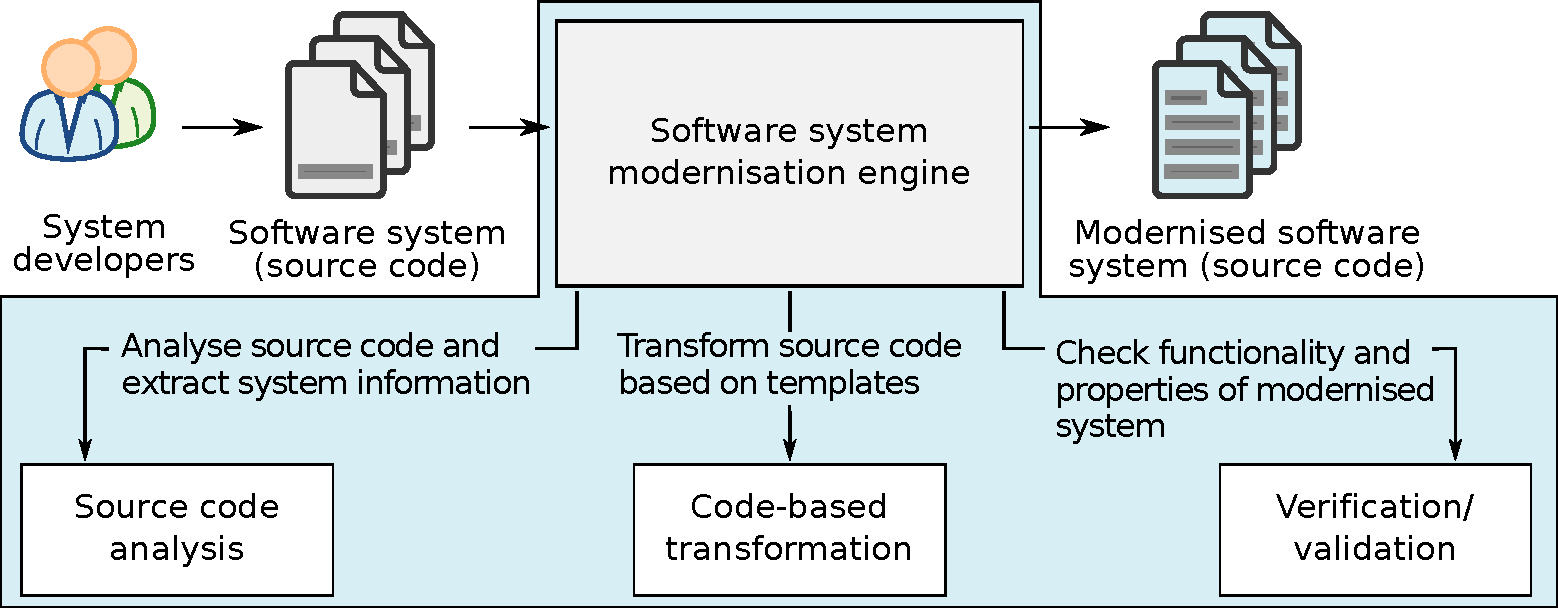
\includegraphics[width=.9\linewidth]{architecture.pdf}
	
	\caption{High-level software modernisation approach.}
	\label{fig:approach}
	
	\vspace*{-2em}
\end{figure}

Through analysing the source code of the software system under consideration, 
we would gain insight into the architecture of the system, including 
interconnections between software modules and dependencies with 
external libraries and components. Furthermore, this code analysis will provide 
useful information on how to best address the obsolescence issues and 
re-architect the software, if needed.

The approach illustrated in Figure~\ref{fig:approach} is based on the use of transformation technology.
Two types of transformations have been used to support rehosting: extraction 
transformations (to ``pull'' abstract specifications from legacy code) and text 
generators, based on templates. The transformations have been implemented using Epsilon, the rich C/C++ parsing and analysis 
infrastructure provided by the Eclipse CDT project, and ANTLR/Xtext to support 
additional languages 
such as Ada. The former for implementing the templates, the latter to extract 
abstract specifications from legacy code, in a form suitable for re-engineering 
and amenable to application of the templates. 
The transformation chain will automatically generate traceability 
information in a standard format (e.g., XML-based). Such information will be potentially useful as
evidence that the rehosted/migrated application would be supportive of Software Level C.
In particular, it could used to demonstrate a partial validity argument, 
i.e., that all statements and expressions in the legacy program are transformed 
to statements and expressions in the retargeted program. 

\subsection{Evidence}
The obsolescence management strategy makes use of a number of techniques to support software migration and rehosting.
These techniques are underpinned by a number of engineering artefacts that can either be used directly as evidence in assurance, or
can be used to \textit{generate} evidence that can be used to support assurance, of the migrated or rehosted software system. 
We are assuming that we are migrating a system that has already undergone some level of certification or assurance,
e.g., against DO-178C or similar standards, to DAL-C or similar. As such, some assurance evidence already exists.

The sources of evidence available to or generated by the obsolescence management strategy and technical approach are as follows.

\begin{itemize}
\item \textit{Tests}: test cases and test evidence will have been produced for the original certification and assurance. Migration and rehosting
is designed to ensure that the migrated software system is behaviourally equivalent (modulo behavioural differences in the hardware platform).
As such, the migrated and rehosted system should satisfy the original test cases.

\item \textit{Traceability}: the technical approach we have developed generates (as a side-effect) traceability information between the original
source program and the target program. In this way, information capturing how source statements have been replaced with target statements has
been captured. This information can be externalised and used to support impact analysis, which in turn will provide information to safety engineers as
to (a) which parts of the software system have changed; (b) which parts have not changed; and (c) where they may need to concentrate their efforts
in re-certifying. Note that traceability information is \textit{static} and \textit{syntactic:} it captures the fact that program statements have been 
transformed into new program statements, but says nothing about the meaning of the transformation.

\item \textit{Transformations:} the rehosting/migration technical approach makes use of transformations and text generation algorithms, which have
been tested and can be further audited and reviewed, in much the same way as a compiler can be tested and reviewed and ultimately qualified (though in Section~\ref{sec:future}
we briefly discuss some of the challenges of qualifying migration tool chains like the one we have developed).
\end{itemize}

In the next section we briefly discuss the impact of migration on relevant safety standards -- particularly  DO-178C -- and analyse the effect of migrating
a software system using the technical approach on any previously existing safety argument and safety process.

\section{Certification and DO-178C Objectives}
In this section we discuss issues associated with migrating a software application where the original system has been certified with respect to  DO-178C,
which are appropriate standard to be used in the development of a legacy airborne system. In particular, what we wish to investigate is the \textit{impact}
of migration on an accomplishment summary. Recall that DO-178C (and DO-178B for that matter) identifies a set of software activities that can take place within the context of a broader 
engineering process, and requires an accomplishment summary \cite{DO178C} as part of the certification deliverables. The accomplishment summary is a 
document that demonstrates compliance of a system with the plan for software aspects of certification. The accomplishment summary in
DO-178C (DO-178B is largely similar at a high levey) requires the following to be addressed:

\begin{enumerate}[(a)]
\item System overview
\item Software overview
\item Certification considerations
\item Software characteristics
\item Software life cycle 
\item Software life cycle data
\item Additional considerations
\item Software identification
\item Change history
\item Software status
\item Compliance statement
\end{enumerate}

The primary safety argument underlies the software life cycle data. This is clear in Annex A of DO-178C, which provides tables of objectives for each of ten areas (DO-178B is largely a subset of these objectives, with some variation in the details, e.g., treatment of Parameter Data Files). The tables are:
\begin{enumerate}
\item Software Planning Process
\item Software Development Process
\item Verification of Outputs of Software Requirements Process
\item Verification of Outputs of Software Design Process
\item Verification of Outputs of Software Coding and Integration Processes
\item Testing of Outputs of Integration Process 
\item Verification of Verification Process Results
\item Software Configuration Management Process
\item Software Quality Assurance Process
\item Certification Liaison Process
\end{enumerate}

Several of the tables map directly to the accomplishment summary, e.g., Table 8 relates to point h, software identification, and Table 10 relates to point c. The majority of tables, i.e. 3-7, are primarily providing support for point f, software life cycle data, in the accomplishment summary. 

So if an accomplishment summary has been produced for a legacy system, and the software application has been migrated, then the accomplishment summary will no longer be valid and accurate for the migrated application. What parts of the accomplishment summary -- i.e., the Objective tables in DO-178C Annex A -- will either be invalidated (and hence require full work) or partially invalidated? We briefly outline the results of our initial analysis. We attempt to indicate if Objectives for DO-178C are \textit{directly} impacted by the application of the migration technology and strategy (and hence substantial work will be required to rebuild an accomplishment summary), and if Objectives are \textit{indirectly} impacted (in which case any rework will hopefully be minor). 

The assumptions that we make in carrying out this analysis are as follows.
\begin{itemize}
\item The original system has been developed according to DO-178C. This may be an unreasonable assumption, given that we are migrating legacy aerospace applications; it may be more reasonable to assume that they had been developed according to DO-178B. However, the similarities between objective tables across the two standards should allow us to make at least an initial analysis.
\item The migrated system is to be certified against DO-178C.
\item The software has been migrated using our technical approach, outlined in the previous section and in \cite{Gerasimou2017};
\item Test cases from the original system are available (and these test cases are automated and executable).
\end{itemize}
We present an initial analysis of the DO-178C objectives. We also briefly touch on the Model-Based Development annexe, and DO-254. The latter two standards are discussed only briefly as the primary focus in the project was on software rehosting and Model-Based Development techniques were not used broadly). All of our analyses are preliminary, 
given the time and resource available to us in the project. It would also be interesting to consider technical migration of accomplishment summaries from DO-178B to DO-178C, but this is a research project in and of itself.

\subsection{DO-178C Assessment}
\label{sec:DO178C}
In this section we briefly analyse the impact of migration against DO-178C objectives.

\subsubsection{Table A-1: Software Planning Process}
Our view is that this table is only indirectly (and lightly) impacted by the application of the migration strategy and approach. There will be one-off costs associated with documenting the new development process associated with the migrated application (which is a combination of the original development process and the application of the obsolescence strategy), setting up the process, explaining it to the certification authority, etc. There may also be process improvement issues as developers become more experienced with the migration approach and can see ways to improve it or extend it. With respect to A-1-7, there is a question as to whether the software plans for the legacy system consider rehosting and migration. If they do not, they should be revised and this process should be coordinated.

\subsubsection{Table A-2: Software Development Processes}
Our view is that this table is indirectly impacted by the application of the migration strategy. We are assuming that the requirements have not changed, and that an architecture is still developed. The most signfiicant impact may be with objective A-2-6 (Source code is developed) -- the migration approach produces new source code, but it is generated automatically rather than manually by an engineer. It may be that documenting the process by which source code is produced is sufficient to convince a certifying authority. A-2-7 is also interesting: we assume the parameter data files are invariant across the legacy and rehosted system. However, if we are interested in qualifying the technical solution itself, ensuring that parameter data files for the solution (i.e., the legacy application itself, as well as any of its parameter data files) will need to be loaded. This is not a difficult issue to deal with, but it does increase the number of artefacts that engineers must manage.

\subsubsection{Table A-3: Verification of Outputs of Software Requirements Process}
This table is indirectly impacted, but it is here that we start to see a greater impact from migration: the impact will be mitigated by reuse of tests to demonstrate that algorithms remain accurate. However, migration to a new hardware platform may affect algorithm accuracy, and so it is questionable whether, in all circumstances, that reused acceptance, integration and system tests will be sufficient to fully demonstrate that the compliance and consistency objectives have been met. If, however, reuse of tests is not possible for whatever reason, this objective will be directly and significantly impacted and all objectives in the table may need to be re-established.

\subsubsection{Table A-4: Verification of Outputs of Software Design Process}
This table may be \textit{directly} impacted, depending on the form of migration: in the case where migration to a new hardware platform, or a new programming language or operating system is involved, there will be direct impact. 

There are similar concerns about algorithm accuracy (A-4-7) as discussed in the previous subsection. The objectives specific to software architecture (i.e., A-4-8 through A-4-13) are directly impacted due to migration, especially A-4-10 (e.g., if the new hardware platform is significantly different to the original, such as in the case of migrating from single core to multicore). In general, if the software architecture from the original system remains unchanged (i.e., behaviourally equivalent components and interfaces) then A-4-8 through A-4-13 (excepting A-4-10) should hold. New evidence will need to be produced to demonstrate that the migrated software architecture is compatible with the target architecture.

\subsubsection{Table A-5: Verification of Outputs of Software Coding and Integration Processes}
\label{sec:a-5}
This table may be \textit{directly} impacted, particularly because this requires demonstration that source code complies with low-level requirements, and new source code has been produced. At worst, this will require a fresh argument to support A-5-1, to show that the migrated code complies with low-level requirements. There may be opportunities to exploit \textit{model weaving} to reduce the effort in this: since we have (from the previous summary) evidence that the original source code complies with requirements, and we have traceability (supplied by the migration strategy) from original to new source code, we envision a process where this evidence and traceability information is woven together. At the very least this could indicate which parts of the original requirements/source code relationship have changed and require re-certification. A similar approach could be used for A-5-5. 

Another issue to consider is independence: if original code is migrated, is the independence (required for A-5-1) lost? Does anything new have to be done to re-establish independence when assuring the migrated code? At worst, independence will have to be entirely re-established if the project is operating at software level A or B.

A-5-8 and A-5-9 are similar to A-1-7 (discussed earlier): we assume that parameter data files do not change due to migration, but there existence adds another level of detail that must be managed in qualification.

%% This one is tricky, especially A-5-5 traceability of code to low-level requirements
%% Also, what about the independence argument for A-5-1 and A-5-2; if you migrate the code does that invalidate the independence from the
%% original, if you are at SW Level A or B? 

\subsubsection{Table A-6: Testing of Outputs of Integration Process}
This table is \textit{directly} impacted by application of the migration strategy, largely because it involves object code that must be produced from source code. As such, objectives A-6-1 through A-6-5 have to be carried out again once new object code has been produced from the new source code. Are there opportunities for reuse of the original safety argument? Perhaps -- the main difficulty will be in producing evidence to show how new object code relates to the original object code (the migration strategy that we have developed generates traceability information only for rehosting of source code; an instrumented compiler would be needed to generate traceability information for object code). If such traceability information could be provided, then a model weaving approach may potentially be applied, similar to what was discussed in Section~\ref{sec:a-5}.

\subsubsection{Table A-7: Verification of Verification Process Results}
This table will be \textit{directly} impacted by migration assuming that test cases (and test procedures etc) from the original application are available. However the direct impact may not be as significant as in some of the previous tables. Assuming that test cases and procedures are reused, then we do not expect objectives A-7-1 through A-7-4 to be affected. However objectives A-7-4 through A-7-8 may have to be re-established as it may be the case that the source code structures have changed as a result of rehosting (e.g., introduction of new control structures due to introduction of a new library or API), and previous MC/DC evidence is no longer valid. However, if it possible to evidence that the source code structures have not changed as a result of migration (which may be the case if it is a like-for-like API replacement), then the previous evidence may remain valid. A-7-9 is very interesting: in general, additional code will be conservatively copied from legacy system to rehosted system, and hence evidence for A-7-9 for the legacy application should still hold. However, it may be possible for the rehosting process to identify such code as a ``bad smell''\footnote{Note: we have not done this in the current project.} so that it can either be removed or appropriate verification can be carried out.

\subsubsection{Table A-8: Software Configuration Management Process}
This table will be \textit{indirectly} affected. The issue here is whether the technical solution to software migration should be supported by the configuration management process. Effectively, does the software life cycle \textit{include} the technical software migration phase, or is this phase assumed to be out of scope? In our view it should be consider in-scope as some of the evidence used to support re-certification (traceability data) is produced by the technical solution. This traceability data must be considered in baselining activities under A-8-2. Additionally, new configuration items related to the components of the technical solution (grammars, parsers, templates, transformations) should also be considered in A-8-1. It may be that the other objectives can remain unchanged.

\subsubsection{Table A-9: Software Quality Assurance Process}
This table is arguably \textit{indirectly} impacted, largely because the software development and integral processes have been modified as a result of using the technical migration solution: new code is produced by applying the technical solution, and it is automatically integrated with existing code that has not changed. These processes need to be shown to comply with software plans and standards. It is not immediately clear if \textit{new} standards need to be considered with respect to the technical solution -- for example, standards for representing evidence produced by the technical solution. It may, for example, be necessary and useful to ensure that traceability evidence generated by the technical solution is compliant with suitable standards -- e.g., the OMG's Structured Assurance Case Metamodel -- even if these have not yet seen widespread use in safety critical projects.

\subsubsection{Table A-10: Certification Liaison Process}
This table is of course \textit{directly} impacted across all objectives as there will be changes made to the production of an accomplishment summary for the migrated code, and the certifying authority will need to be informed and will need to buy-in to the new processes. Given that certifying authorities are increasingly aware of DO-178C (and, for example, the model-based design annexe, which is aimed at supporting lifecycles with some similarity to our technical solution), this may be less problematic and challenging today than it was several years ago.

Table~\ref{table:summary} summarises the objectives and the impact that rehosting may have on them.

\begin{table}[htbp]
\begin{center}
\begin{tabular}{|c|c|c|}\hline\hline
\textbf{Objective Table} & \textbf{Direct Impact} & \textbf{Indirect Impact} \\ \hline
A-1 & & $\surd$ \\ \hline
A-2 & & $\surd$ \\ \hline
A-3 & & $\surd$ \\ \hline
A-4 & $\surd$ & \\ \hline
A-5 & $\surd$ & \\ \hline
A-6 & $\surd$ & \\ \hline
A-7 & $\surd$ & \\ \hline
A-8 & & $\surd$ \\ \hline
A-9 & & $\surd$ \\ \hline
A-10 & $\surd$ & \\ \hline\hline
\end{tabular}
\end{center}
\caption{Summary of DO-178C objective tables and how they are impacted by the migration approach}
\label{table:summary}
\end{table}

\subsubsection{Model-Based Development Supplement}
One issue that we have not considered in detail is applicability of and conformance to the Model-Based Development (MBD) supplement of DO-178C. The supplement specifically aims to address usage of principled and automated abstractions in expressing requirements, producing code (i.e., code generation) and tracing requirements through to code. The technical solution produced in this project is, broadly, not a model-based development approach to rehosting, as it operates on source code. However, it does follow some of the principles of MBD -- e.g., the use of abstract internal representations (ASTs), the use of structured code generation technology (templates), and the use of modelling tools (Epsilon) to implement the toolchain. As such, certification of a migrated application under DO-178C following the MBD supplement is a promising route forward.

\subsubsection{DO-254 Analysis}
The focus of the project has been on software migration, and developing technical solutions to the challenges of software rehosting. However, one of the experiments has briefly considered hardware migration in a restricted form, focusing on software API remapping that is needed when replacing hardware components (e.g., changes in sensors). As a result of these experiments we can briefly comment on the impact of rehosting on different aspects of the DO-254 \textit{lifecycle}, as to where significant effort may be required as a result of migration.

The DO-254 lifecycle is summarised in Figure~\ref{fig:DO254}.

\begin{figure}[htbp]
	\vspace*{-2em}
	\centering
	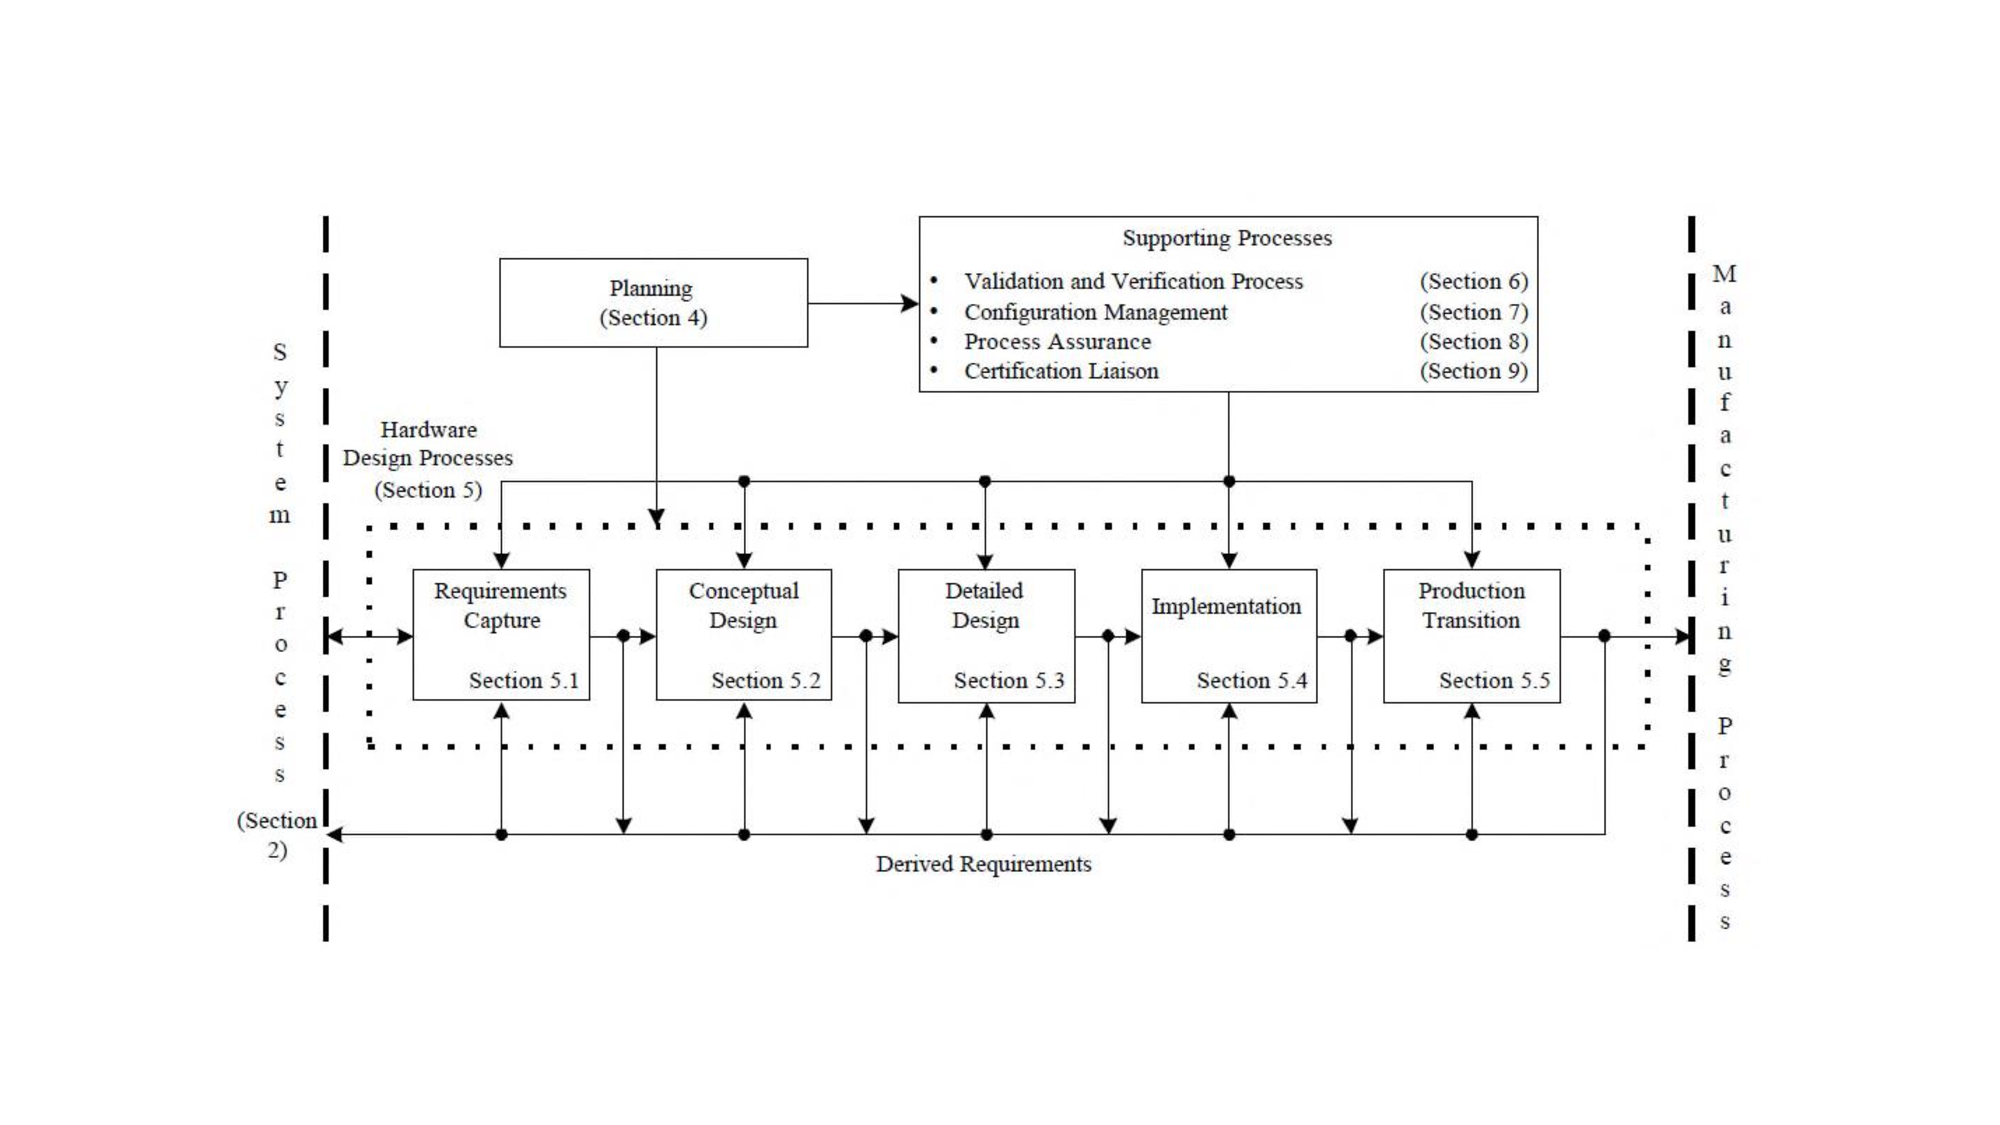
\includegraphics[width=1.1\linewidth]{DO254.pdf}
	
	\caption{DO-254 lifecycle, taken from \cite{DO254}.}
	\label{fig:DO254}
	
	\vspace*{-2em}
\end{figure}

With respect to the key phases in Figure~\ref{fig:DO254}, we observe the following.

\begin{itemize}
\item The \textit{System Process} (DO-254 Section 2) is unlikely to be impacted as the DAL level should remain the same after rehosting, and the derived requirements should
not change.

\item The \textit{Planning Process} (DO-254 Section 4) will change as the plan for hardware aspects of certification will be impacted by the new hardware (whether it is new components or a new processor). Given the importance of the PHAC and the need for agreement on it with the certifying authority, it is very important that sufficient resource be allocated to this activity.

\item The \textit{Requirements Capture} (DO-254 Section 5.1) task is unlikely to be impacted, as we can assume that a sensible requirements capture mechanism has been established for the legacy project.

\item The \textit{Conceptual Design} (DO-254 Section 5.2) task may be impacted, depending on the extent of the hardware changes. If the changes involve replacing like-with-like (i.e., behavioural similar/identical component replacement) then there will be no impact. A wholesale processor change may result in the need for a conceptual redesign, however.

\item The \textit{Detailed Design} (DO-254 Section 5.3) will be impacted, as it must take into account the new hardware components and/or processors as well as any additional design (e.g., FPGA design). 

\item The textit{Implementation} (DO-254 Section 5.4) may not be impacted if there is only component replacement, but no new design (i.e., FPGA or VHDL code).

\item We did not consider \textit{Production Transition}.

\item The \textit{Validation and Verification} (DO-254 Section 6) will be impacted in terms of verification and in terms of traceability, i.e., that requirements are traceable to their implementation. It may be that some of the traceability information from the legacy application can be reused (because some of the hardware design may not change).

\item \textit{Configuration Management} (DO-254 Section 7) is unlikely to be impacted as it should be possible to reuse what was developed for the legacy project.

\item \textit{Process Assurance} (DO-254 Section 8) should be unchanged, assuming that the project role was identified in the legacy project.

\item \textit{Certification Liaison} (DO-254 Section 9) should be unaffected, assuming that engagement with the certifying authority was established for the legacy project.
\end{itemize}

\section{The Future: Tool Qualification and Assurance Case Generation}
In this section we briefly explore two issues that have not been considered at all in this project -- tool qualification and assurance case generation -- and posit on some of the difficulties associated with their use in the future.

\subsection{Tool Qualification}
The technical solution that has been produced in this project automates otherwise manual processes (e.g., API rewriting). As such, and according to SC-205/WG-71, assurance should be obtained that the technical solution is at least as dependable as the manual approach. 

DO-178C defines three criteria that determine the applicable tool qualification level (TQL); one is relevant to the technical solution that has been produced in this project:

\begin{quotation}
\textbf{Criteria 1:} A tool whose output is part of the airborne software and thus could insert an error.
\end{quotation}
Criteria 2 relates to verification processes (which are not considered by the technical solution), whereas Criteria 3 relates to failure of detection of errors. We do not believe that Criteria 3 is relevant as it is focused on verification tools. As such, Criteria 1 is relevant to the technical solution. If the qualification criterion for the software application being rehosted is Level C, then the applicable TQL is level 3: the replacement of DO-178B development tool for each software level.

With respect to DO-330/ED-215 \cite{DO330}, there are a number of considerations related to tool qualification for the technical solution. 

Firstly, the operational environment for the technical solution needs to be established. This needs to meet specific objectives related to installing the technical solution in the appropriate environment, showing that the tool requirements are compatible with the operational environment, etc. It should be observed that the technical solution has been developed in an iterative and incremental manner, in close collaboration with DSTL, and as such a rigorous requirements specification for the tool has not been produced. As such, additional future work will need to be carried out on this. This should likely include the \textit{Tool Operational Requirements (TOR)} (i.e., Section~10.3.1 of DO-330). 

The TOR for the technical solution that has been produced is complicated, in part because the tool has interfaces with other tools, particularly Eclipse, which has a plug-in architecture. Eclipse is a very substantial piece of software that can be customised for different purposes. The technical obsolescence strategy has relied on Eclipse CDT (a set of tools for development of C/C++, including parsers) and Eclipse Epsilon (a set of tools for code generation and transformation). Capturing the tool functions and technical features will be challenging because of the generality of Eclipse. As well, capturing abnormal activation modes for the technical solution will be challenging as some of these will also depend on activation modes for Eclipse and for its sub-projects. With specific reference to DO-330, we make the following points.

\begin{itemize}
\item The Tool Operational Requirements for the technical solution developed in this project will need to capture interfaces with other tools. At the most conservative level this will need to capture: Eclipse CDT (which provides the parser support for the C/C++ input languages), Eclipse Epsilon (which provides the template-based programming language), ANTLR (which is used internally by Epsilon for parser support), Eclipse itself, and Java.

\item The TOR can reuse definitions of input files, as these are expected to be standards-compliant C or C++.

\item The TOR can largely reuse definitions of output files, as these are also expected to be standards-compliant C or C++. However, it is also possible to output \textit{trace links} (in the form of an XML representation) and this should be captured as well.

\item Abnormal activation modes in the TOR should consider parser failure (e.g., on erroneous or malformed C/C++ input), exceptions within the execution of the Eclipse tooling, and malformed output (e.g., C/C++ that does not parse). It may be possible to construct an argument that the technical solution only produces C/C++ code that does not lead to abnormal activation modes (specifically, that the solution produces C/C++ code that is syntactically well-formed and does not lead to an error in the execution of the tool - though this does not guarantee that the C/C++ code produced by the solution is valid). Abnormal activation modes may also need to consider how the software vulnerabilities identified in \cite{Burns2017} are checked.

\item Production of DO-330 Tool Requirements (as opposed to TOR) will be more expensive as this will require description of all tool functions and features. What is challenging here is that Eclipse provides a wealth of functions and features, many of which are not used by the technical solution. Thus, qualification of the solution may need to consider partitioning into features of Eclipse (and Epsilon) that are ``in scope'' and features that are out of scope.

\item Tool robustness is likely to require additional tests to be crafted, in order to demonstrate coverage of inputs. In the testing carried out in the project, we have not fully carried out robustness testing, e.g., as to whether the technical solution produces a sensible output for all potential input C/C++ program.

\item The user interface for Eclipse may provide extraneous features (extraneous in terms of effort in obtaining tool qualification, but not in terms of usability of the solution). As such, producing a headless version of the technical solution may be useful. This is generally not difficult to do.
\end{itemize}

We envision a larger research program to assess the challenges and difficulties of tool qualification within the Eclipse ecosystem, and suggest collaboration with Polarsys\footnote{\url{www.polarsys.org}} to support this. We note that the costs associated with tool qualification of Eclipse-based tools have not been thoroughly investigated by the research community, and collaboration with other partners with similar concerns would be a reasonable way to mitigate risk and control costs.

\subsection{Assurance Case Generation}
Part of the process of assuring a migrated/rehosted software system is to develop (or revise) an assurance or safety case, e.g., represented using GSN or a similar notation. In an ideal situation it would be feasible to carry out an impact analysis on an assurance case, after rehosting, in order to identify what has changed within an argument structure. This would require, for example, traceability information to have been recorded between the assurance case and the original system artefacts (e.g., source code, architecture and design models, tests). It is unlikely to be able to find such information easily in legacy projects -- some is implicit, some will be scattered across multiple documents, some will be tacit. As such, an impact analysis will largely be a manual process. Using the technical solution developed in this project will help with this, as traceability information will be recorded between original and migrated code, but the links with the legacy assurance or safety case will likely not be available.

In terms of future proofing and making the technical solution more useful going forward, we can suggest an approach to \textit{assurance case generation} from engineering artefacts, including source code, design models and architectures. The approach described in \cite{HASE15} shows how to generate outline/template assurance cases from artefacts through the use of weaving models, which are based on traceability information.  This approach is compatible with what the technical solution developed in this project has produced, but some further infrastructure would need to be produced to represent traceability information as a weaving model. The approach would not generate a complete assurance or safety case, but a template that engineers could complete (much as the technical solution developed in this project does not generate a complete migrated application). 

The idea with automatically generating assurance cases is to ensure that all the information required to support future impact analyses is recorded and persisted, and to reduce the amount of effort required to update a safety case in the future. Unfortunately it was not possible to investigate the generation of assurance cases in this project, but some aspects of this are being explored in the ATI-funded project SECT-AIR.

\section{Conclusions}
We have highlighted an initial perspective on the key ``pain points'' for certification or re-certification of a software application that has been rehosted using the technical solution developed in this project. The analysis indicates where effort may need to be focused on re-certification under either DO-178C or DO-178B. We have also commented on the applicability of the Model-Based Development supplement to DO-178C, the challenges of tool qualification, and the role that automated generation of outline assurance cases could play in the future.

Two interesting questions arise, which DSTL may wish to consider in its future research and development, pertaining to rehosting and certification:
\begin{enumerate}
\item To what extent is it possible to \textit{migrate} an accomplishment summary from DO-178B to DO-178C? It may be that the technical solution developed in this project can play a role in supporting this.

\item Can the use of the Model-Based Development supplement ease the recertification costs, given that the technical solution developed in this project can be treated as a Model-Based Development approach?
\end{enumerate}

\bibliographystyle{abbrv}
\bibliography{bibliography}
\renewcommand{\baselinestretch}{1.0}


\end{document}